\chapter{Reinforcement Learning Method}

\section{Reinforcement Learning}

In reinforcement learning our goal is to train a agent such that he finds the optimal policy $\pi(s)$.
This means that the agent finds the best possible action $a$ in each game state $s$.


\begin{figure}[H]
	\centering
    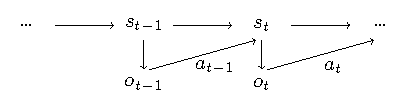
\includegraphics[scale=1.5]{fig//rl_diagram.pdf}
	\caption{Diagram for reinforcement learning}
	\label{img:Q-table}
\end{figure}


\section{Q-Learning}

We used Q-Learning for our agent.
The general Idea for Q-learning is to find the expected reward (or Q-values) for each action that the agent perform in a given
game-state.
If the space of states is small we could compute a matrix that would contain all Q-values.
In each Game-state we would then take a look at the Matrix and pick the action that gives the highest expected reward.


\begin{figure}[H]
	\centering
    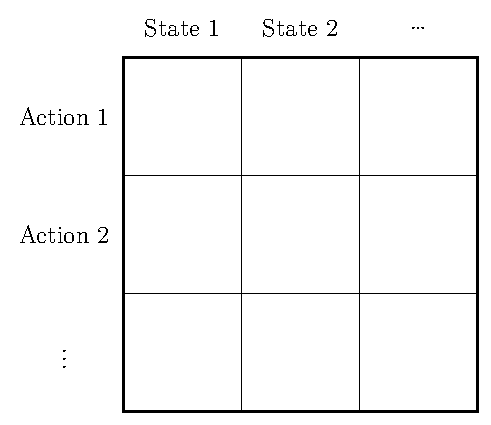
\includegraphics[scale=.8]{fig//q_table.pdf}
	\caption{Q-table}
	\label{img:Q-table}
\end{figure}

The Q-Values can be computed in the following way:
\begin{align}
    \hat{Q}(s_t, a_t) = \hat{Q}_{\text{current}} + \alpha (y_t + \hat{Q}_{\text{current}} (s_t, a_t))
\end{align}
In the first round the Q-Value will just be the reward that a specific action gave, but as the training continues the Q-values get more and more precise.
The definition of $y_t$ is different from algorithm to algorithm.
At the beginning of our work we started with a 1-Step Q-learning algorithm.
It's called 1-Step because we only use the expected reward of the next round.
$y_t$ is then defined as:
\begin{align}
y_t = R_{t+1} + \gamma \ \underset{a'}{\max}  \hat{Q}_{\text{current}}(s_{t+1}, a')
\end{align}

However, later on we moved to a n-step algorithm. 
As the name suggests, one computes the expected reward of the next $n$ steps.
In this case $y_t$ is given as:

\begin{align}
    y_t = \sum_{t'=t+1}^{t+n} \gamma^{t' - t -1} R_t + \gamma^n \hat{Q}_{\text{current}} (s_{t+n}, a_{t+n})
\end{align}


Unfortunately for us the number of states in Bomberman is far to big to use this strategy.
What we do instead of calculating the entries of the Q-table is to define features which we use to characterize a game state.
We define Q-functions that take these features as input and output our Q-function.
So we shifted the problem from getting all Q-values to getting only some Q-values and fitting curves.

\section{Regression Model}

We need six different Q-functions for each of the possible actions (left, right, up, down, wait and bomb).
In our case these Q-functions are linear functions, that take the features $x_i$ and the parameters $\theta_{i, a}$ and output our guess for the Q-value:
\begin{align}
    q_\theta (a, x_1, \dots , x_n) = \theta_{0,a} + \theta_{1,a} x_1 + \dots + \theta_{n,a} x_n
\end{align}
where $n$ is the number of features. 
Because $x_1, \dots, x_n $ describe our state $s$ we will write $q_\theta (a, s)$ in the following.\\

In order to get the best possible parameters $\hat{\theta}_{i, a}$ we need to solve the following optimization problem:
\begin{align}
    \hat{theta} = \underset{\theta}{\text{argmin}} \ \mathcal{L}(q_\theta (a,s), Q^\ast (a,s))
\end{align}
Here $Q^\ast (a,s) $ are the meassured Q-values and $\mathcal{L}(q_\theta (a,s), Q^\ast (a,s))$ is the Loss function which is defined as:
\begin{align}
    \mathcal{L} = \sum_t ( \underbrace{\mu}_{weight} y_t - q_\theta (a_t , s_t) )^2. 
\end{align}

\subsection{Levenberg Marquardt}

We solved this optimization problem by using the Levenberg Marquardt Algorithm











